% B4.9 -- backup appendix
\appendix
\setsecblurb{Raw material behind the claims.}
\section{Backup}

\begin{frame}[t]{Backup --- \Eone, the raw \dt\ sweep}
  \begin{columns}[T]
    \begin{column}{0.52\textwidth}
      \footnotesize
      \begin{tabular}{@{}crrrr@{}}
        \toprule
        \thead{\dt\ (min)} & \thead{acc \%} & \thead{conf \%} & \thead{gap} & \thead{visual tokens} \\
        \midrule
        \TabEoneSweep
        \bottomrule
      \end{tabular}
      \vskip0.5em
      {\footnotesize Bin-1 accuracy \EoneBinOneAcc\,\% sits \EoneRange\ pp above the no-evidence floor of \EoneFloorAcc\,\%. Any statement about an accuracy \emph{level} is made inside that narrow band.}
    \end{column}
    \begin{column}{0.45\textwidth}
      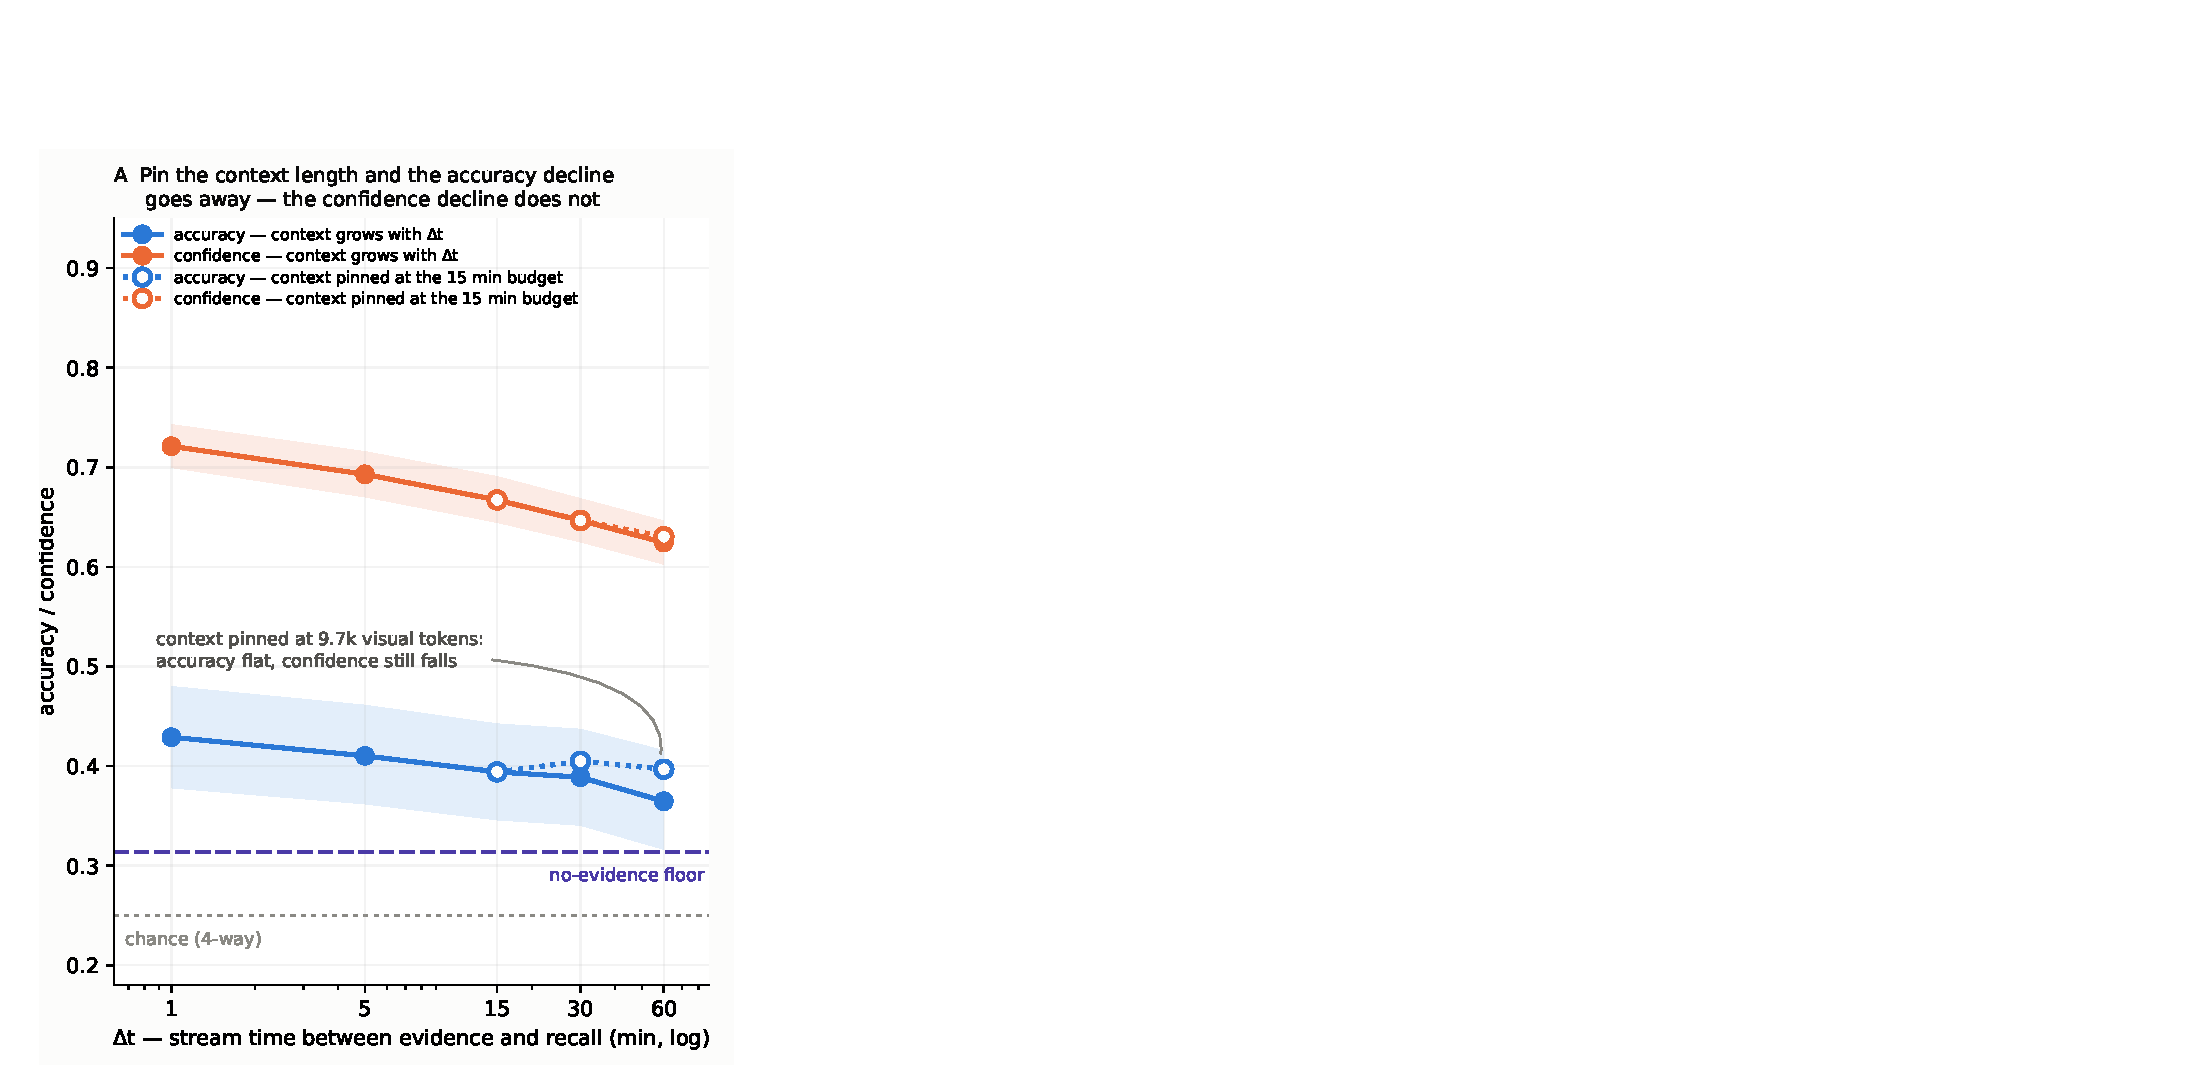
\includegraphics[width=\textwidth,height=0.72\textheight,keepaspectratio]{figures/e1-a.pdf}
    \end{column}
  \end{columns}
\end{frame}

\begin{frame}[t]{Backup --- the decomposition, in both regimes}
  \begin{columns}[T]
    \begin{column}{0.53\textwidth}
      \footnotesize
      \begin{tabular}{@{}lrr@{}}
        \toprule
        \thead{\Eone: \dt\ 15\,$\rightarrow$\,60 min} & \thead{\acc{acc}} & \thead{\conf{conf}} \\
        \midrule
        elapsed-time term & \EoneDecompAccElapsed\ pp & \EoneDecompConfElapsed\ pp \\
        context-length term & \EoneDecompAccContext\ pp & \EoneDecompConfContext\ pp \\
        \bottomrule
      \end{tabular}
      \vskip0.5em
      {\footnotesize Accuracy's decline is entirely the context term; confidence's is almost entirely elapsed time.}
      \vskip0.4em
      {\footnotesize \Etwo: \conf{\EtwoDecompConfContext\ pp} of context against \conf{\EtwoDecompConfElapsed\ pp} of elapsed time, observed \EtwoDecompConfObs\ pp, residual \EtwoDecompResid\ pp.}
    \end{column}
    \begin{column}{0.45\textwidth}
      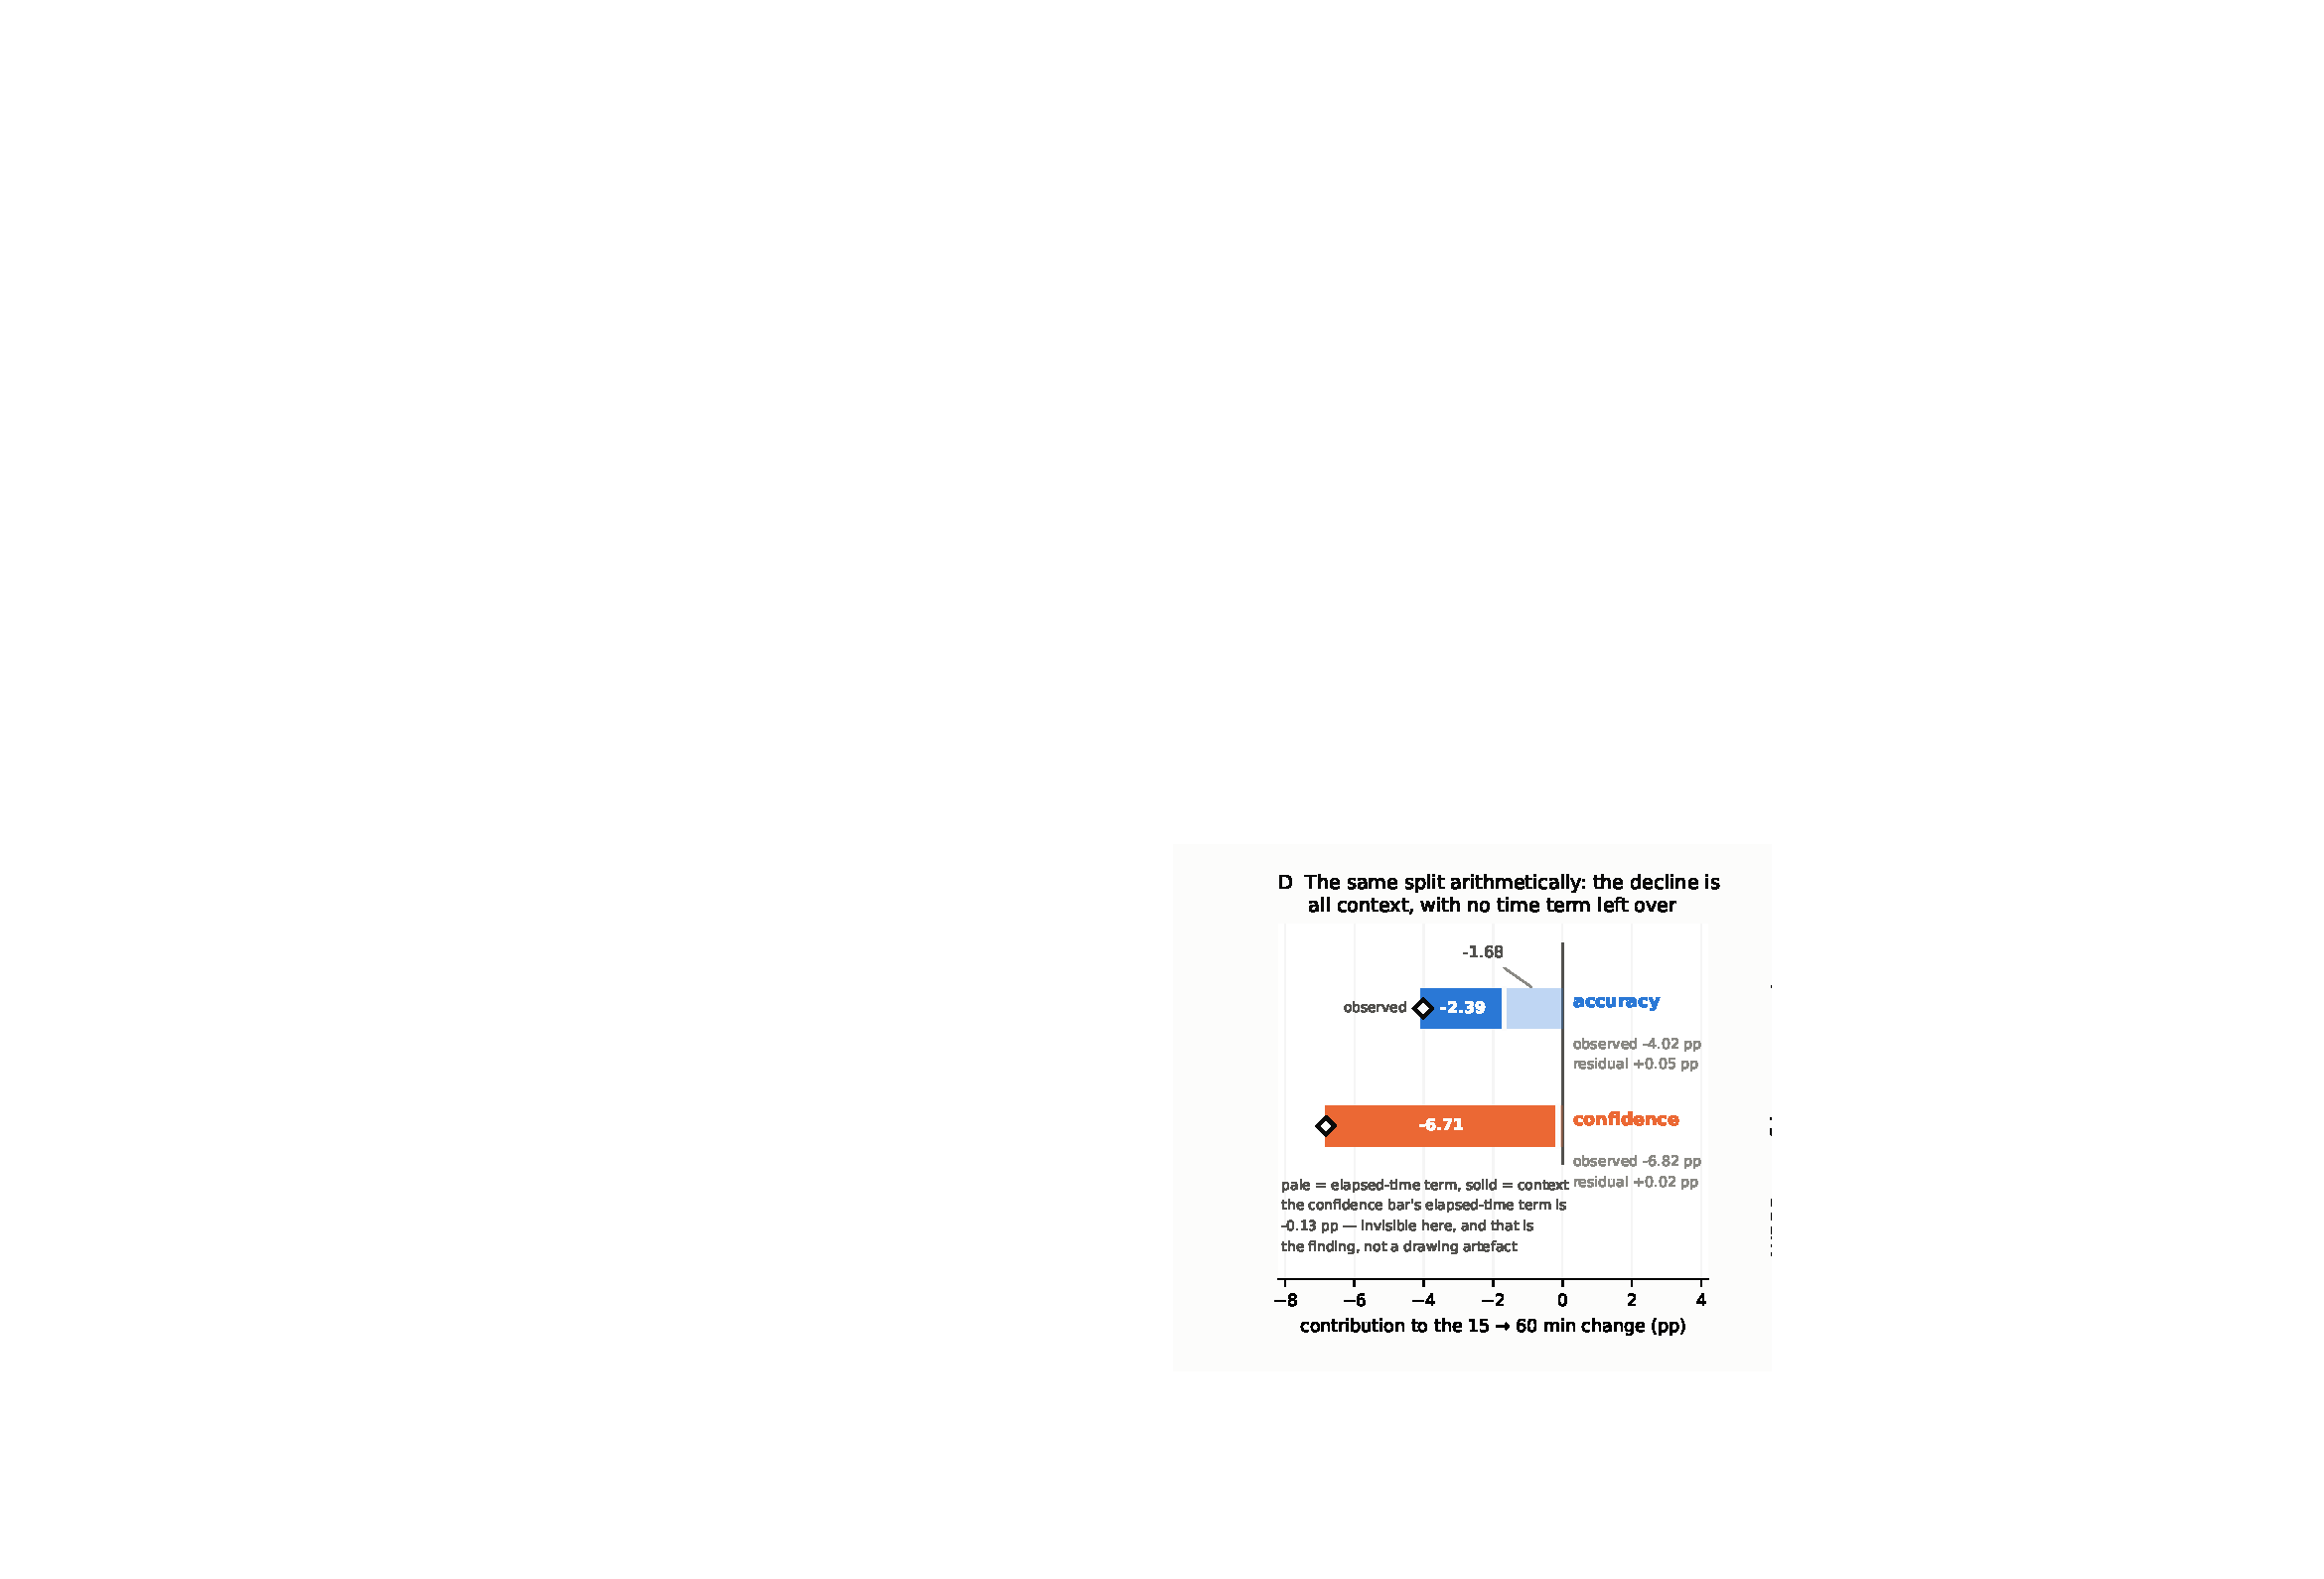
\includegraphics[width=\textwidth]{figures/e2-d.pdf}
    \end{column}
  \end{columns}
\end{frame}

\begin{frame}[t]{Backup --- \Etwo, the whole headline figure}
  \begin{center}
    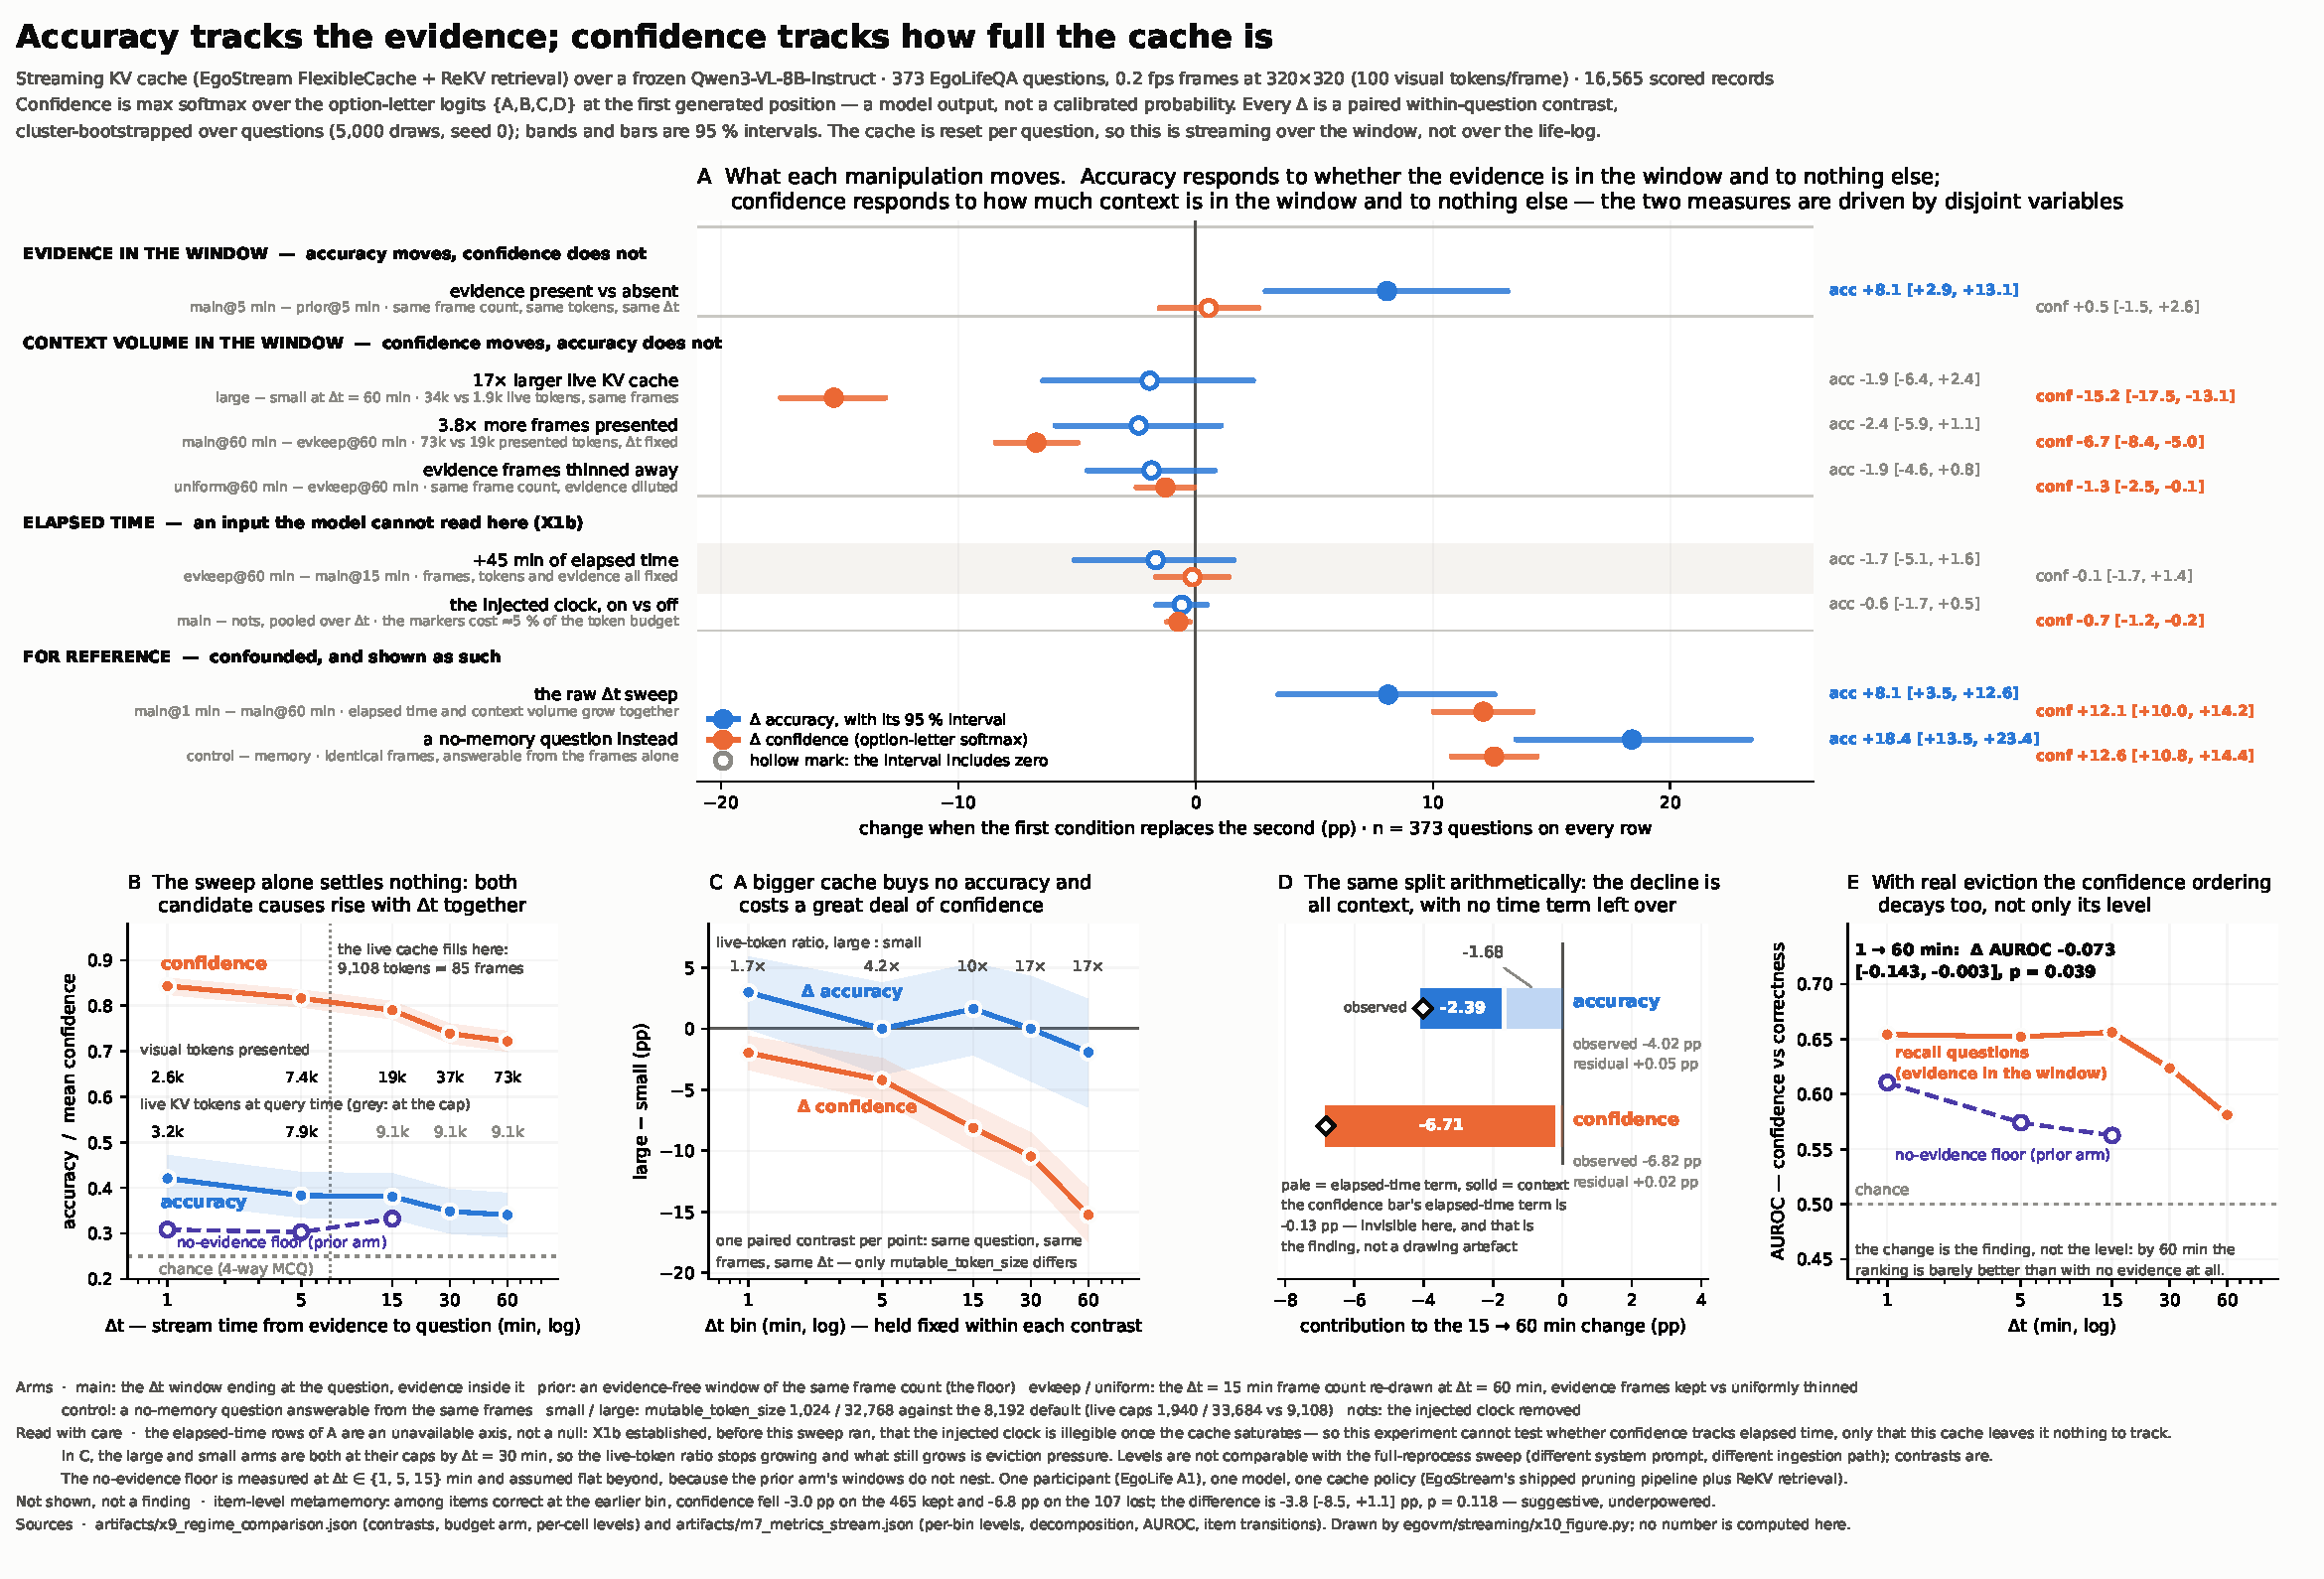
\includegraphics[width=\textwidth,height=0.80\textheight,keepaspectratio]{figures/e2-full.pdf}
  \end{center}
\end{frame}

\begin{frame}[t]{Backup --- \Etwo, full streaming contrasts}
  \begin{center}\footnotesize
    \begin{tabular}{@{}p{6.4cm}rr@{}}
      \toprule
      \thead{manipulation} & \thead{\acc{$\Delta$accuracy}} & \thead{\conf{$\Delta$confidence}} \\
      \midrule
      evidence in context vs none & \EtwoEvidenceAcc & \EtwoEvidenceConf \\
      $+$45 min elapsed, frames and evidence fixed & \EtwoElapsedAcc & \EtwoElapsedConf \\
      3.8$\times$ more presented tokens & \EtwoFourxAcc & \EtwoFourxConf \\
      \CleanBudgetRatio\ live-token budget (offload-free pair, 60 min) & \emph{\CleanBudgetAcc} & \CleanBudgetConf \\
      17$\times$ live-token budget (spans the offload boundary) & \EtwoBudgetAcc & \EtwoBudgetConf \\
      evidence frames thinned away & \EtwoThinnedAcc & \EtwoThinnedConf \\
      injected clock on vs off & \EtwoTimestampsAcc & \EtwoTimestampsConf \\
      \midrule
      raw \dt\ sweep \emph{(confounded)} & \EtwoRawAcc & \EtwoRawConf \\
      no-memory vs recall \emph{(between-items)} & \EtwoKindAcc & \EtwoKindConf \\
      \bottomrule
    \end{tabular}
  \end{center}
  \source{\texttt{artifacts/x9\_streaming.md}, generated from \texttt{x9\_regime\_comparison.json}.}
\end{frame}

\begin{frame}[t]{Backup --- three readings to rule out}
  \begin{enumerate}\footnotesize\setlength\itemsep{0.5em}
    \item \textbf{``The elapsed-time effect disappeared under streaming.''} No. EgoStream's image path carries no time markers; the injected clock is unreadable once the cache saturates. The axis is \textbf{unavailable}, not null.
    \item \textbf{``Streaming makes the model more overconfident.''} Not supported --- that is a level comparison, and the regime changes the system prompt and ingestion path. Contrasts are comparable; levels are not.
    \item \textbf{``The model tracks the items it actually lost.''} Not yet. \Etwo's kept-vs-lost difference is \EtwoItemDiff, $p$ = \EtwoItemDiffP, on \EtwoItemLost\ lost items --- suggestive, underpowered.
  \end{enumerate}
  \vskip0.4em
  \claim{\scriptsize Calling an \textbf{unavailable} axis a \textbf{null} is the most damaging misreading here --- a reviewer will make it if the paper does not pre-empt it.}
\end{frame}

\begin{frame}[t]{Backup --- where EgoSAT appears to contradict, and why it does not}
  \begin{columns}[T]
    \begin{column}{0.49\textwidth}
      {\footnotesize\textbf{1. Confidence does not fall with distance in their table} (\EgosatSixOfEight\ slopes).}
      \vskip0.3em
      {\footnotesize Against \Etwo: consistent but uninformative --- neither evidence state nor token count changes between their three probes, so their flat slope is the expected null, not a replication. Against \Eone: apparent disagreement, for three estimand differences (45 min vs 16 s; slope fitted on all-correct items only; no intervals).}
    \end{column}
    \begin{column}{0.49\textwidth}
      {\footnotesize\textbf{2. Their accuracy declines with distance} (\EgosatAccDecline\ over 8\,$\rightarrow$\,24 s) \textbf{where our token-matched arms say elapsed time costs no accuracy.}}
      \vskip0.3em
      {\footnotesize Their lag axis is uncontrolled for context volume. Their streaming models show the smallest or non-monotone declines --- matching our account.}
    \end{column}
  \end{columns}
  \vskip0.4em
  {\scriptsize The defensible framing: their uncontrolled lag axis reproduces our uncontrolled raw sweep --- and this project has the control that separates the components.}
\end{frame}

\begin{frame}[t]{Backup --- what the cache actually holds}
  \begin{columns}[T]
    \begin{column}{0.52\textwidth}
      {\footnotesize The cache: pinned priming region, evictable mutable region (the budget knob), protected hat (last two frames). On overflow, the pruning pipeline drops the lowest-value and most redundant tokens.}
      \vskip0.4em
      {\footnotesize Eviction is content-scored and global, not recency-ordered. ``Older evidence is pushed out first'' is not this policy. Eviction is permanent in the primary condition: \OffloadDefault\ default/large rows offloaded anything, against \OffloadSmall\ small rows.}
    \end{column}
    \begin{column}{0.45\textwidth}
      \claim{\scriptsize The sweep crosses saturation at \SaturationPoint. By \dt\ = 60 min only \SurvivingShare\ of the presented tokens survive, live tokens pinned at \LiveTokensIdentical\ from 15 min on.}
      \vskip0.5em
      {\scriptsize \Eone's clock is \emph{text} the model tokenizes (\EoneClockIsText), not a positional encoding --- confirmed by decoding the prompt through \Eone's own input builder.}
    \end{column}
  \end{columns}
  \source{\texttt{memo/STREAMING-CACHE.md} \S2, \S6--\S7.}
\end{frame}

\begin{frame}[t]{Backup --- dataset curation: 500 $\rightarrow$ 373 questions}
  \begin{columns}[T]
    \begin{column}{0.52\textwidth}
      \footnotesize
      \begin{tabular}{@{}p{3.8cm}rrl@{}}
        \toprule
        \thead{step} & \thead{in} & \thead{out} & \thead{reason} \\
        \midrule
        EgoLifeQA A1 (full) & 500 & --- & \\
        Drop TaskMaster & 500 & 437 & prospective \\
        Screen HabitInsight & 437 & 376 & no single anchor \\
        Evidence span $>$\,15\,min & 376 & 373 & ambiguous \dt \\
        \bottomrule
      \end{tabular}
      \vskip0.4em
      {\footnotesize\textbf{What survives.} EntityLog\,/\,EventRecall\,/\,RelationMap at 125\,/\,124\,/\,124. Answer letters 83\,:\,96\,:\,97\,:\,97. All 373 appear in every \dt\ bin and every arm; no per-bin attrition.}
      \vskip0.25em
      {\footnotesize\textbf{Token matching.} Matched arms hold visual tokens exactly at the \dt\,=\,15\,min level (mean 9,679) across all bins. Prior arms frame-matched to \texttt{main} with zero difference.}
      \vskip0.25em
      {\footnotesize\textbf{Flagged, not dropped.} \texttt{need\_audio}\,=\,true on 110/373 (29.5\,\%); results reported with and without.}
    \end{column}
    \begin{column}{0.45\textwidth}
      {\footnotesize\textbf{Why the drops are defensible.}}
      \vskip0.25em
      {\footnotesize\textbf{TaskMaster} (63): questions about future plans --- incompatible with a retrospective \dt\ sweep. 93.7\,\% require audio; the vision-only model is near-blind on them independently.}
      \vskip0.25em
      {\footnotesize\textbf{HabitInsight} (61): habitual patterns with no single evidence event to anchor \dt. Scored separately, not dropped.}
      \vskip0.25em
      {\footnotesize\textbf{Span exclusions} (3): q482 spans 50.7\,h (3 evidence points across two days; alone 13\,\% of frame-encodes). q189/q346 at 19/21\,min. Next-closest is 11.6\,min --- clean gap below the 15\,min threshold.}
      \vskip0.25em
      \claim{\scriptsize 96.5\,\% have a single evidence point (span\,=\,0). The span filter affects a small tail; ``\dt\ since evidence'' is unambiguous for the rest.}
    \end{column}
  \end{columns}
  \source{M1 \texttt{m1\_questions.py}, M4 \texttt{m4\_plan.py}; verified from \texttt{m1\_questions.jsonl} and \texttt{m4\_eval\_plan.jsonl}.}
\end{frame}

\begin{frame}[t]{Backup --- how this deck is built}
  \footnotesize
  \begin{tabular}{@{}llp{6.0cm}@{}}
    \toprule
    \thead{module} & \thead{artifact} & \thead{checks} \\
    \midrule
    B1 \texttt{b1\_numbers.py} & \texttt{generated/numbers.tex} & Re-derives all macros from metrics JSON; memo-sourced values carry a literal check. \\
    B2 \texttt{b2\_figures.py} & \texttt{figures/*.pdf} & Panels are crops; manifest pins source figures by sha256. \\
    B5 \texttt{b5\_verify.py} & the built PDF & Nine checks: stale generators, missing figures, undefined macros, LaTeX errors, overfull slides. \\
    \bottomrule
  \end{tabular}
  \vskip0.5em
  {\footnotesize No number on any slide was typed by hand. If an experiment is re-run, \texttt{make} rebuilds the deck and \texttt{make verify} fails until it is rebuilt.}
\end{frame}
